まずフォームによる送信の例を見てみましょう。以下のようなフォームのコンテンツがあるとします。login.gtplというファイルを新規作成します。(新しくディレクトリを作ってその中に入れてください)

\begin{lstlisting}[numbers=none]
<html>
<head>
<title></title>
</head>
<body>
<form action="/login" method="post">
    ユーザ名:<input type="text" name="username">
    パスワード:<input type="password" name="password">
    <input type="submit" value="ログイン">
</form>
</body>
</html>
\end{lstlisting}

上で送信されるフォームはサーバの\texttt{/login}に渡されます。ユーザが情報を入力しログインをクリックした後、サーバのルーティングの\texttt{login}にリダイレクトします。まずはこの送信が何のメソッドによるものか判断する必要があります。POSTでしょうかGETでしょうか?

httpパッケージにはそれを取得するとても簡単な方法があります。前のwebの例を基礎にloginページのformデータをどのように処理するか見てみましょう。



\begin{lstlisting}[numbers=none]
package main

import (
    "fmt"
    "html/template"
    "log"
    "net/http"
    "strings"
)

func sayhelloName(w http.ResponseWriter, r *http.Request) {
    r.ParseForm()       //urlが渡すオプションを解析します。
                        //POSTに対してはレスポンスパケットの
                        //ボディを解析します(request body)
    //注意:もしParseFormメソッドがコールされなければ、
    // 以下でフォームのデータを取得することができません。
    //これらのデータはサーバのプリント情報に出力されます
    fmt.Println(r.Form)
    fmt.Println("path", r.URL.Path)
    fmt.Println("scheme", r.URL.Scheme)
    fmt.Println(r.Form["url_long"])
    for k, v := range r.Form {
        fmt.Println("key:", k)
        fmt.Println("val:", strings.Join(v, ""))
    }
    fmt.Fprintf(w, "Hello astaxie!")
    //ここでwに書き込まれたものがクライアントに出力されます。
}

func login(w http.ResponseWriter, r *http.Request) {
    fmt.Println("method:", r.Method) //リクエストを取得するメソッド
    if r.Method == "GET" {
        t, _ := template.ParseFiles("login.gtpl")
        t.Execute(w, nil)
    } else {
        //ログインデータがリクエストされ、
        //ログインのロジック判断が実行されます。
        fmt.Println("username:", r.Form["username"])
        fmt.Println("password:", r.Form["password"])
    }
}

func main() {
    //アクセスのルーティングを設定します
    http.HandleFunc("/", sayhelloName)
    //アクセスのルーティングを設定します
    http.HandleFunc("/login", login)
    //監視するポートを設定します
    err := http.ListenAndServe(":9090", nil)
    if err != nil {
        log.Fatal("ListenAndServe: ", err)
    }
}
\end{lstlisting}

上のコードにおいてリクエストのメソッドを取得するには\texttt{r.Method}だけで済むことがわかります。これは文字列型の変数です。GET, POST, PUT等のmethod情報を返します。

login関数では\texttt{r.Method}に従ってログイン画面を表示するのかログインロジックを処理するのかが判断されます。GETメソッドによるリクエストの場合はログイン画面を表示し、その他のメソッドによるリクエストではログインロジックを処理します。例えばデータベースを検索したり、ログイン情報を検証したりといった事です。

ブラウザで\texttt{http://127.0.0.1:9090/login}を開いた時に以下のような画面が現れます。

\begin{figure}[H]
  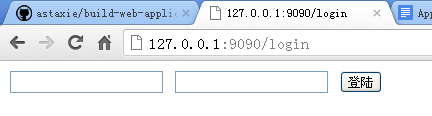
\includegraphics[width=14cm]{4.1.login.png}
   \label{図4.1}
   \caption{ユーザログイン画面}
\end{figure}

我々がユーザ名とパスワードを入力してもサーバは何も出力しません。なぜでしょうか?デフォルトではHandlerの中ではformの内容を自動的に解析しないからです。必ず明示的に\texttt{r.ParseForm()}をコールした後でなければ、このフォームのデータに対して操作を行うことはできません。コードを少し修正して、\texttt{fmt.Println("username:", r.Form["username"])}の前に\texttt{r.ParseForm()}という一行を追加してください。再コンパイルしてもう一度入力、送信してみると、今度はサーバがあなたの入力したユーザ名とパスワードを出力するはずです。

\texttt{r.Form}では全てのリクエストのデータが含まれています。例えばURLの中のquery-string、POSTのデータ、PUTのデータなどです。URLのquery-stringフィールドとPOSTが衝突する場合はsliceに保存されます。これには複数の値が保存されています。Goのオフィシャルドキュメントでは次のバージョンでPOST、GETといったデータは分離されると述べています。

ではlogin.gtplのformのaction値である\texttt{http://127.0.0.1:9090/login}を\texttt{http://127.0.0.1:9090/login?username=astaxie}に変更してもういちど試してみましょう。サーバが出力するusernameはsliceになっていませんか。サーバの出力は以下のようになります:

\begin{figure}[H]
  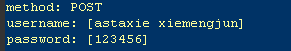
\includegraphics[width=7cm]{4.1.slice.png}
   \label{図4.1}
   \caption{サーバが受け取ったデータを表示}
\end{figure}

\texttt{request.Form}はurl.Values型です。この中には\texttt{key=value}のような対応するデータが保存されています。ここではformデータに対していくつかの操作をご紹介します:

\begin{lstlisting}[numbers=none]
v := url.Values{}
v.Set("name", "Ava")
v.Add("friend", "Jess")
v.Add("friend", "Sarah")
v.Add("friend", "Zoe")
// v.Encode() == "name=Ava&friend=Jess&friend=Sarah&friend=Zoe"
fmt.Println(v.Get("name"))
fmt.Println(v.Get("friend"))
fmt.Println(v["friend"])
\end{lstlisting}

\begin{quote}
\textbf{Tips}: RequestそのものもFormValue()関数でユーザが送信したデータを取得できます。例えばr.Form["username"]はr.FormValue("username")とも書けます。r.FormValueをコールした時は自動的にr.ParseFormがコールされますので、事前にコールする必要はありません。r.FormValueは同名のデータの中から一つ目のものだけを返します。もしデータが存在しない場合は空文字列を返します。
\end{quote}


